\documentclass{beamer}

\beamertemplatenavigationsymbolsempty

\usepackage{graphicx}
\usepackage{hyperref}
\usepackage{booktabs}

\usepackage{tikz}
\usetikzlibrary{calc}

\newcommand{\NH}{\text{NH}}
\newcommand{\RG}{\text{RG}}

\title{Emergent Behaviour}
\author{Vince Knight}
\date{2015-11-11}

\begin{document}

\frame{\titlepage}

\frame{
    \Huge
    \[
        \begin{pmatrix}
        (3,3)&(0,5)\\
        (5,0)&(1,1)
        \end{pmatrix}
    \]
}

\frame{
    \begin{center}
        \includegraphics[width=.8\textwidth]{static/axelrod.pdf}
    \end{center}
}


\frame{
\begin{center}
    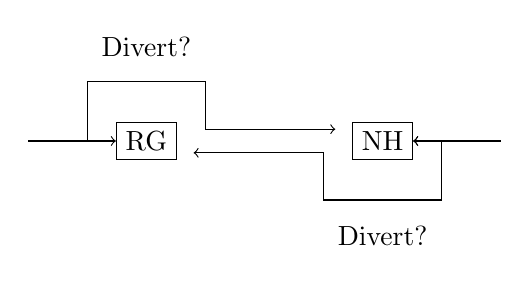
\begin{tikzpicture}[scale=1.5]
        \node (A) at (0,0) [draw] {RG};
        \node (B) at (2,0) [draw] {NH};
        \draw [->] (-1,0) -- (A);
        \draw [->] (3,0) -- (B);
        \draw [->] (-1,0) -- ($(A)+(-.5,0)$) -- ($(A)+(-.5,.5)$) -- ($(A)+(.5,.5)$) -- ($(A)+(.5,.1)$) -- ($(B)+(-.4,.1)$);
        \draw [->] (3,0) -- ($(B)+(.5,0)$) -- ($(B)+(.5,-.5)$) -- ($(B)+(-.5,-.5)$) -- ($(B)+(-.5,-.1)$) -- ($(A)+(.4,-.1)$);
        \draw [->] (3,0) -- (B);
        \node at ($(A) + (0,.8)$) {Divert?};
        \node at ($(B) + (0,-.8)$) {Divert?};
    \end{tikzpicture}
\end{center}
}

\frame{
\begin{center}
\includegraphics[width=.8\textwidth]{./static/argminPoAmodel2.pdf}
\end{center}
}

\frame{
    \begin{center}
    \only<1>{\includegraphics[width=\textwidth]{static/basic_network.pdf}}
    \only<2>{\includegraphics[width=\textwidth]{static/network_with_center.pdf}}
    \only<3>{\includegraphics[width=\textwidth]{static/spanning_tree.pdf}}
    \end{center}
}

\frame{
    \begin{center}
        \Huge{Investigating Social Networks with Agent Based Simulation and Link
        Prediction Methods}
        \flushright{\small{Angelico Fetta}}
    \end{center}
}

\frame{
            \begin{center}
                \includegraphics[width=\textwidth]{static/link_prediction.pdf}
            \end{center}


            \pause

            \begin{center}
                \tiny
            \begin{tabular}{llll}
                \toprule
                Pair        & Adamic Adar & Preferentiel Attachment & Resource Allocation\\
                \midrule
                \((1, 3)\)    & 1.632       & 0.583                   & 6 \\
                \((1, 4)\)    & 1.721       & 0.250                   & 8 \\
                \bottomrule
            \end{tabular}
        \end{center}


}

\frame{
    \frametitle{Python Tools}
    \begin{itemize}
        \item Game Theoretic analysis: Gambit, Sagemath, Axelrod
        \item Network Analysis: Networkx
    \end{itemize}
}
\end{document}
